% =====================================================================
% NBA Text-to-SQL — COSI 115b Final Presentation
% Author: Zixin (Stan) Wan
%
% Build:
%   pdflatex presentation_slides.tex
%   pdflatex presentation_slides.tex   % run twice for ToC / refs if needed
%
% Recommended theme is "metropolis" (modern, included in TeX Live 2017+).
% If your TeX distribution does not have it, replace
%     \usetheme{metropolis}
% with
%     \usetheme{Madrid}
% and remove the \metroset{...} line below.
% =====================================================================

\documentclass[aspectratio=169,11pt]{beamer}

\usetheme{metropolis}
\metroset{
  block=fill,
  numbering=fraction,
  progressbar=frametitle,
  sectionpage=progressbar,
}

\usepackage[english]{babel}
\usepackage[T1]{fontenc}
\usepackage[utf8]{inputenc}
\usepackage{microtype}
\usepackage{booktabs}
\usepackage{array}
\usepackage{multirow}
\usepackage{tikz}
\usepackage{pgfplots}
\pgfplotsset{compat=1.17}
\usepackage{listings}
\usepackage{xcolor}
\usepackage{amsmath}
\usepackage{appendixnumberbeamer}

\usetikzlibrary{positioning, arrows.meta, shapes.geometric, fit, backgrounds}

% ---------- Colors ----------
\definecolor{nbaBlue}{HTML}{1D428A}
\definecolor{nbaRed}{HTML}{C8102E}
\definecolor{accentGreen}{HTML}{2E7D32}
\definecolor{lightGray}{HTML}{F2F2F2}
\definecolor{midGray}{HTML}{B0B0B0}

\setbeamercolor{alerted text}{fg=nbaRed}
\setbeamercolor{progress bar}{fg=nbaBlue}
\setbeamercolor{title separator}{fg=nbaBlue}
\setbeamercolor{frametitle}{bg=nbaBlue, fg=white}

% ---------- Listings (SQL) ----------
\lstdefinelanguage{prettySQL}{
  morekeywords={SELECT, FROM, WHERE, GROUP, BY, ORDER, LIMIT, AS, AND, OR,
    COUNT, AVG, SUM, JOIN, ON, HAVING, DISTINCT, CASE, WHEN, THEN, ELSE, END},
  sensitive=false,
  morecomment=[l]{--},
  morestring=[b]',
}
\lstset{
  language=prettySQL,
  basicstyle=\ttfamily\footnotesize,
  keywordstyle=\color{nbaBlue}\bfseries,
  stringstyle=\color{accentGreen},
  commentstyle=\color{midGray}\itshape,
  showstringspaces=false,
  breaklines=true,
  columns=fullflexible,
  frame=single,
  rulecolor=\color{midGray},
  framerule=0.4pt,
  xleftmargin=2pt,
  xrightmargin=2pt,
}

% ---------- Title ----------
\title{Retrieval-Augmented Text-to-SQL with PEFT for Cross-Domain NBA Analytics}
\subtitle{COSI 115b -- Fundamentals of NLP II -- Final Presentation}
\author{Zixin (Stan) Wan}
\institute{Brandeis University}
\date{May 6, 2026}

\begin{document}

% =====================================================================
\begin{frame}[plain]
  \titlepage
\end{frame}

% =====================================================================
\begin{frame}{Agenda}
  \tableofcontents[hideallsubsections]
\end{frame}

% =====================================================================
\section{Task, Track \& Focus}
% =====================================================================

\begin{frame}{Task and Motivation}
  \begin{block}{What we are building}
    An end-to-end \textbf{text-to-SQL} system that turns natural-language
    NBA questions into executable queries on a real SQLite database.
  \end{block}

  \begin{columns}[T,onlytextwidth]
    \column{0.55\textwidth}
      \textbf{Why it matters}
      \begin{itemize}
        \item Analytics workflows are blocked by schema literacy.
        \item NBA is a compact yet realistic, schema-rich target domain.
        \item Cross-domain transfer is the practical pain point: train broad,
              deploy narrow.
      \end{itemize}
    \column{0.45\textwidth}
      \begin{exampleblock}{Concrete example}
        \textbf{Q:} ``Which team had the highest average home points
        in the 2022--23 regular season?''\\[3pt]
        \textbf{SQL:}\\
        {\footnotesize\ttfamily SELECT team\_name\_home, AVG(pts\_home)
          FROM game WHERE season\_id='22022' \dots}
      \end{exampleblock}
  \end{columns}
\end{frame}

% =====================================================================
\begin{frame}{Track and Focus}
  \begin{columns}[T,onlytextwidth]
    \column{0.5\textwidth}
      \begin{alertblock}{Track: Applied}
        Runnable end-to-end pipeline with a live demo and held-out
        evaluation -- not just an offline benchmark.
      \end{alertblock}
      \begin{alertblock}{Focus: Training}
        Depth on \emph{adaptation regimes}, \emph{LoRA rank sweep}, and
        an \emph{adaptation-data ablation} \(n \in \{0, 10, 20, 70, \text{all}\}\).
      \end{alertblock}
    \column{0.5\textwidth}
      \textbf{Why this combination?}
      \begin{itemize}
        \item Two practical questions drive every design choice:
          \begin{enumerate}
            \item Which PEFT strategy gives the best transfer trade-off?
            \item Does schema retrieval (RAG) help downstream SQL?
          \end{enumerate}
        \item Single-GPU compute budget $\rightarrow$ PEFT is the only
              feasible path for breadth of ablation.
      \end{itemize}
  \end{columns}
\end{frame}

% =====================================================================
\section{Approach: Data, Model, Baseline}
% =====================================================================

\begin{frame}{System Pipeline}
  \centering
  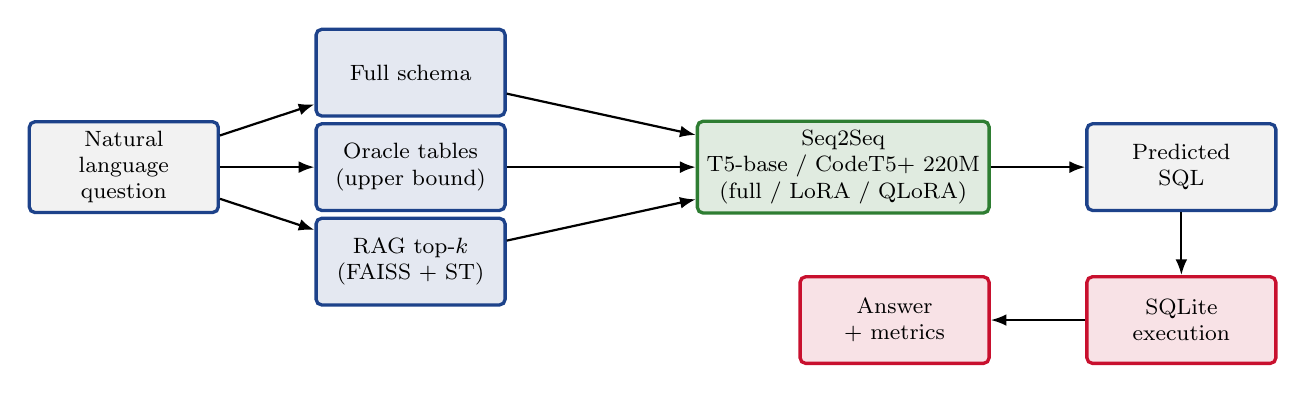
\begin{tikzpicture}[
    node distance=10mm and 12mm,
    box/.style={draw=nbaBlue, very thick, rounded corners=2pt,
                fill=lightGray, minimum width=24mm, minimum height=11mm,
                align=center, font=\footnotesize},
    schema/.style={box, fill=nbaBlue!12},
    model/.style={box, fill=accentGreen!15, draw=accentGreen},
    output/.style={box, fill=nbaRed!12, draw=nbaRed},
    arr/.style={-{Latex[length=2mm]}, thick},
  ]
    \node[box] (q) {Natural\\language\\question};

    \node[schema, right=of q, yshift=12mm] (full)   {Full schema};
    \node[schema, right=of q]              (oracle) {Oracle tables\\(upper bound)};
    \node[schema, right=of q, yshift=-12mm](rag)    {RAG top-$k$\\(FAISS + ST)};

    \node[model, right=24mm of oracle] (m)
      {Seq2Seq\\T5-base / CodeT5+ 220M\\(full / LoRA / QLoRA)};

    \node[box, right=of m] (sql) {Predicted\\SQL};
    \node[output, below=8mm of sql] (db)  {SQLite\\execution};
    \node[output, left=of db]       (ans) {Answer\\+ metrics};

    \draw[arr] (q) -- (full);
    \draw[arr] (q) -- (oracle);
    \draw[arr] (q) -- (rag);
    \draw[arr] (full)   -- (m);
    \draw[arr] (oracle) -- (m);
    \draw[arr] (rag)    -- (m);
    \draw[arr] (m) -- (sql);
    \draw[arr] (sql) -- (db);
    \draw[arr] (db)  -- (ans);
  \end{tikzpicture}

  \vspace{4pt}
  {\footnotesize The schema-context branch (full / oracle / RAG) is the
  knob exercised in every ablation.}
\end{frame}

% =====================================================================
\begin{frame}{Data and Split Protocol}
  \begin{columns}[T,onlytextwidth]
    \column{0.5\textwidth}
      \textbf{Spider (source domain)}
      \begin{itemize}
        \item \texttt{xlangai/spider}, 10{,}181 questions, 200 DBs.
        \item Used for source-domain pretraining of every backbone.
      \end{itemize}

      \textbf{NBA (target domain)}
      \begin{itemize}
        \item Real \texttt{nba-sql} SQLite DB.
        \item 200 authored question / SQL pairs.
        \item Difficulty: easy / medium / hard / extra\_hard.
      \end{itemize}
    \column{0.5\textwidth}
      \begin{block}{Deterministic 150 / 50 split}
        Stored in \texttt{data/nba/nba\_split.json}.\\[2pt]
        Every reported number uses \texttt{--split test}, eliminating leakage
        across runs.
      \end{block}
      \begin{block}{Adaptation budgets}
        $n \in \{0, 10, 20, 70, 150\}$ NBA training examples,
        used to draw the cross-domain transfer curve.
      \end{block}
  \end{columns}
\end{frame}

% =====================================================================
\begin{frame}{Methods}
  \begin{columns}[T,onlytextwidth]
    \column{0.5\textwidth}
      \textbf{Backbones}
      \begin{itemize}
        \item T5-base (220M)
        \item CodeT5+ 220M
      \end{itemize}

      \textbf{Training regimes}
      \begin{itemize}
        \item Full fine-tuning (\texttt{--method full})
        \item LoRA, ranks $r \in \{4, 8, 16\}$
        \item QLoRA (4-bit + LoRA)
      \end{itemize}
    \column{0.5\textwidth}
      \textbf{Adaptation pipeline}\\
      Spider checkpoint $\rightarrow$ continue training on NBA train
      partition with $n \in \{0,10,20,70,\text{all}\}$.

      \textbf{Inference modes}
      \begin{itemize}
        \item Full schema
        \item \alert{Oracle tables} -- retrieval upper bound
        \item \alert{RAG top-$k$} -- FAISS + sentence-transformers
      \end{itemize}

      \textbf{Metrics}: execution accuracy (primary), exact match.
  \end{columns}
\end{frame}

% =====================================================================
\begin{frame}{Baselines (per rubric)}
  \centering\small
  \begin{tabular}{lcc}
    \toprule
    \textbf{System} & \textbf{Exec acc} & \textbf{Exact match} \\
    \midrule
    Zero-shot T5-base prompt           & 0.00 & 0.00 \\
    Few-shot  T5-base prompt           & 0.00 & 0.00 \\
    Full T5-base, Spider only (oracle) & 0.04 & 0.00 \\
    LoRA T5-base $r{=}16$, Spider only & 0.04 & 0.02 \\
    \alert{LoRA CodeT5+ $r{=}16$, $n{=}\text{all}$ NBA} & \alert{\textbf{0.46}} & \alert{\textbf{0.42}} \\
    \bottomrule
  \end{tabular}

  \vspace{6pt}
  {\footnotesize Held-out NBA test split, $n = 50$ examples (oracle mode).}

  \begin{exampleblock}{Take-away}
    Prompting alone is insufficient on this schema; the best system improves
    execution accuracy by $\approx 12\times$ over the strongest baseline.
  \end{exampleblock}
\end{frame}

% =====================================================================
\section{Results and Findings}
% =====================================================================

\begin{frame}{Spider Controls (training-side sanity check)}
  \begin{columns}[T,onlytextwidth]
    \column{0.55\textwidth}
      \centering\small
      \begin{tabular}{lc}
        \toprule
        \textbf{Run} (200-ex Spider slice) & \textbf{Exact match} \\
        \midrule
        LoRA CodeT5+ $r{=}16$              & \textbf{0.290} \\
        Full T5-base                       & 0.265 \\
        QLoRA T5-base                      & 0.140 \\
        LoRA T5-base $r{=}16$              & 0.120 \\
        LoRA T5-base $r{=}4$               & 0.070 \\
        LoRA T5-base $r{=}8$               & 0.000 \\
        \bottomrule
      \end{tabular}
    \column{0.45\textwidth}
      \begin{block}{Why it matters}
        \begin{itemize}
          \item CodeT5+ is the strongest source-domain backbone in our regime.
          \item LoRA $r{=}16$ on CodeT5+ \emph{outperforms} full fine-tuning
                of T5-base on the same slice.
          \item Justifies promoting CodeT5+ to the headline NBA experiments.
        \end{itemize}
      \end{block}
  \end{columns}

  \vspace{4pt}
  {\footnotesize Source: \texttt{eval/spider\_summary.csv}. Execution accuracy on this
  short Spider protocol is 0 across the board (a known artifact of the small
  unseen-DB slice), so the comparison is driven by exact match.}
\end{frame}

% =====================================================================
\begin{frame}{Main NBA Results (held-out test, $n{=}50$)}
  \centering\footnotesize
  \begin{tabular}{llccc}
    \toprule
    \textbf{Model} & \textbf{Method} & \textbf{NBA $n_{\text{train}}$} & \textbf{Exec} & \textbf{Exact} \\
    \midrule
    T5-base       & Full       & 0     & 0.04 & 0.00 \\
    T5-base       & LoRA $r{=}16$ & 0     & 0.04 & 0.02 \\
    T5-base       & QLoRA      & 0     & 0.02 & 0.00 \\
    CodeT5+ 220M  & LoRA $r{=}16$ & 0     & 0.10 & 0.00 \\
    \midrule
    T5-base       & LoRA $r{=}16$ & all (150) & 0.16 & 0.16 \\
    \alert{CodeT5+ 220M} & \alert{LoRA $r{=}16$} & \alert{all (150)} & \alert{\textbf{0.46}} & \alert{\textbf{0.42}} \\
    \bottomrule
  \end{tabular}

  \vspace{6pt}
  Source: \texttt{eval/results\_summary.csv} (oracle mode).

  \begin{alertblock}{Headline}
    The best configuration is \textbf{LoRA on CodeT5+ 220M with full NBA
    adaptation in oracle-schema mode}, reaching execution accuracy 0.46.
  \end{alertblock}
\end{frame}

% =====================================================================
\begin{frame}{Most Interesting Finding: Adaptation Curve}
  \centering
  \begin{tikzpicture}
    \begin{axis}[
        width=0.78\textwidth, height=0.55\textheight,
        xlabel={NBA adaptation training examples ($n$)},
        ylabel={Exec accuracy (test, $n{=}50$)},
        xtick={0,10,20,70,150},
        xticklabels={0,10,20,70,all},
        ymin=0, ymax=0.55,
        ytick={0,0.1,0.2,0.3,0.4,0.5},
        legend pos=north west,
        legend style={font=\footnotesize, draw=midGray},
        grid=both,
        major grid style={lightGray},
        minor grid style={lightGray!50},
        tick label style={font=\footnotesize},
        label style={font=\footnotesize},
    ]
      \addplot+[mark=*, very thick, color=accentGreen]
        coordinates {(0,0.10) (10,0.00) (20,0.12) (70,0.26) (150,0.46)};
      \addlegendentry{CodeT5+ 220M LoRA $r{=}16$}

      \addplot+[mark=square*, very thick, color=nbaBlue]
        coordinates {(0,0.04) (10,0.00) (20,0.04) (70,0.08) (150,0.16)};
      \addlegendentry{T5-base LoRA $r{=}16$}
    \end{axis}
  \end{tikzpicture}

  \begin{alertblock}{Take-away}
    \textbf{Adaptation data dominates method choice.} The single $n{=}70
    \rightarrow n{=}\text{all}$ jump (\(+0.20\) on CodeT5+) is larger than any
    method-only gap on Spider-only checkpoints.
  \end{alertblock}
\end{frame}

% =====================================================================
\begin{frame}{RAG Ablation: where the system breaks}
  \centering
  \begin{tikzpicture}
    \begin{axis}[
        ybar,
        bar width=10pt,
        width=0.85\textwidth, height=0.5\textheight,
        ylabel={Exec accuracy},
        symbolic x coords={Oracle, RAG k=1, RAG k=3, RAG k=5},
        xtick=data,
        ymin=0, ymax=0.55,
        ytick={0,0.1,0.2,0.3,0.4,0.5},
        nodes near coords,
        nodes near coords style={font=\scriptsize},
        legend style={font=\footnotesize, draw=midGray, at={(0.98,0.95)}, anchor=north east},
        enlarge x limits=0.18,
        tick label style={font=\footnotesize},
        label style={font=\footnotesize},
    ]
      \addplot+[fill=accentGreen!70, draw=accentGreen]
        coordinates {(Oracle,0.46) (RAG k=1,0.12) (RAG k=3,0.08) (RAG k=5,0.08)};
      \addlegendentry{CodeT5+ 220M, $n{=}\text{all}$}

      \addplot+[fill=nbaBlue!60, draw=nbaBlue]
        coordinates {(Oracle,0.16) (RAG k=1,0.04) (RAG k=3,0.04) (RAG k=5,0.02)};
      \addlegendentry{T5-base, $n{=}\text{all}$}
    \end{axis}
  \end{tikzpicture}

  \begin{alertblock}{Take-away}
    Generation quality is fine; \textbf{retrieval is the bottleneck}. Replacing the
    oracle table list with FAISS top-$k$ collapses exec accuracy by $\approx 4\times$.
    Source: \texttt{eval/rag\_ablation.csv}.
  \end{alertblock}
\end{frame}

% =====================================================================
\begin{frame}{Error Analysis (best vs.\ RAG)}
  \centering\small
  \begin{tabular}{lcc}
    \toprule
    \textbf{Error class} & \textbf{Oracle, $n{=}\text{all}$} & \textbf{RAG $k{=}3$, $n{=}\text{all}$} \\
    \midrule
    Correct          & \textbf{46\%} & 8\% \\
    Schema linking   & 6\%           & \alert{\textbf{78\%}} \\
    Structural       & 18\%          & 6\% \\
    Value grounding  & 30\%          & 8\% \\
    \bottomrule
  \end{tabular}

  \vspace{4pt}
  {\footnotesize Rule-based taxonomy from \texttt{src/error\_analysis.py};
  source: \texttt{eval/error\_analysis\_summary.json}.}

  \begin{block}{Difficulty-stratified picture (best system)}
    Easy 12/17 correct \,\,$\bullet$\,\, Medium 9/17 \,\,$\bullet$\,\,
    Hard 2/13 (mostly value / structural) \,\,$\bullet$\,\, Extra-hard 0/3.
  \end{block}

  \begin{alertblock}{Diagnosis}
    Under RAG, errors flip from value/structural mistakes to overwhelming
    schema-linking failures -- generation is healthy, retrieval is not.
  \end{alertblock}
\end{frame}

% =====================================================================
\begin{frame}[fragile]{Concrete Failure Example (value grounding)}
  \textbf{Question:} ``How many players are currently active?''

  \vspace{4pt}
  \textbf{Gold:}
\begin{lstlisting}
SELECT COUNT(*) FROM player WHERE is_active = 1;
\end{lstlisting}

  \textbf{Predicted (best system):}
\begin{lstlisting}
SELECT COUNT(*) FROM player
\end{lstlisting}

  \begin{block}{What this tells us}
    Structural skeleton is correct, but the model drops the
    domain-specific literal (\texttt{is\_active = 1}). This is the
    dominant residual failure mode at the high end of our system and
    motivates value-aware decoding for the next iteration.
  \end{block}
\end{frame}

% =====================================================================
\section{Demo, Reproducibility, Next Steps}
% =====================================================================

\begin{frame}{Demo and Reproducibility}
  \begin{columns}[T,onlytextwidth]
    \column{0.5\textwidth}
      \textbf{Live demo}
      \begin{itemize}
        \item \texttt{python -m src.demo}
        \item Question $\to$ SQL $\to$ executed answer.
      \end{itemize}

      \textbf{Reproducibility}
      \begin{itemize}
        \item Deterministic 150/50 NBA split.
        \item Per-run \texttt{run\_config.json} (seed, lr, ranks).
        \item One-command matrix runner:\\
              \texttt{src/run\_experiment\_matrix.py}.
        \item Auto-generated tables: \\
              \texttt{eval/results\_summary.\{csv,md\}}.
      \end{itemize}
    \column{0.5\textwidth}
      \textbf{Single-GPU compute scope}
      \begin{itemize}
        \item All experiments run on one GPU.
        \item PEFT lets us cover full-FT, LoRA r$\in\{4,8,16\}$, QLoRA,
              and a 5-point adaptation curve in one budget.
      \end{itemize}

      \textbf{Repo layout}
      \begin{itemize}
        \item \texttt{src/} -- training, eval, RAG, demo.
        \item \texttt{data/nba/} -- DB + split + QA.
        \item \texttt{eval/} -- raw JSONs + auto-summaries.
        \item \texttt{reports/} -- write-up + slides.
      \end{itemize}
  \end{columns}
\end{frame}

% =====================================================================
\begin{frame}{What I Learned and What's Next}
  \begin{columns}[T,onlytextwidth]
    \column{0.5\textwidth}
      \textbf{What worked}
      \begin{itemize}
        \item PEFT (LoRA) + domain adaptation: best single design choice.
        \item CodeT5+ as the seq2seq backbone for SQL generation.
        \item Oracle-mode upper bound for clean retrieval-vs-generation
              attribution.
      \end{itemize}

      \textbf{What did not}
      \begin{itemize}
        \item Dense-only RAG retrieval -- collapses exec accuracy.
        \item Extra-hard slice still unsolved (0/3).
        \item Single-seed reporting -- no CIs yet.
      \end{itemize}
    \column{0.5\textwidth}
      \begin{alertblock}{Most interesting finding}
        Once a competent backbone is fixed, \textbf{adaptation data is
        the dominant lever}, not method choice or schema breadth.
      \end{alertblock}
      \textbf{Next steps}
      \begin{enumerate}
        \item Hybrid retriever (dense + sparse) and re-ranker.
        \item Value-aware constrained decoding for literal grounding.
        \item Multi-seed runs with confidence intervals.
        \item Expand the NBA benchmark beyond 200 pairs.
      \end{enumerate}
  \end{columns}
\end{frame}

% =====================================================================
\begin{frame}[standout]
  Thank you.\\[6pt]
  {\normalsize Questions?}\\[10pt]
  {\footnotesize Repo: \texttt{nba-text2sql} \quad$\bullet$\quad
   Q\&A prep: \texttt{reports/presentation\_qa.md}}
\end{frame}

% =====================================================================
\appendix
% =====================================================================

\begin{frame}{Backup: full results table (NBA test, oracle)}
  \centering\scriptsize
  \begin{tabular}{llcccc}
    \toprule
    \textbf{Model} & \textbf{Method} & \textbf{$n$} & \textbf{Mode} & \textbf{Exec} & \textbf{Exact} \\
    \midrule
    T5-base       & Full           & 0   & oracle & 0.04 & 0.00 \\
    T5-base       & LoRA $r{=}4$   & 0   & oracle & 0.02 & 0.00 \\
    T5-base       & LoRA $r{=}8$   & 0   & oracle & 0.00 & 0.00 \\
    T5-base       & LoRA $r{=}16$  & 0   & oracle & 0.04 & 0.02 \\
    T5-base       & QLoRA          & 0   & oracle & 0.02 & 0.00 \\
    CodeT5+ 220M  & LoRA $r{=}16$  & 0   & oracle & 0.10 & 0.00 \\
    T5-base       & LoRA $r{=}16$  & 10  & oracle & 0.00 & 0.00 \\
    CodeT5+ 220M  & LoRA $r{=}16$  & 10  & oracle & 0.00 & 0.00 \\
    T5-base       & LoRA $r{=}16$  & 20  & oracle & 0.04 & 0.02 \\
    CodeT5+ 220M  & LoRA $r{=}16$  & 20  & oracle & 0.12 & 0.06 \\
    T5-base       & LoRA $r{=}16$  & 70  & oracle & 0.08 & 0.04 \\
    CodeT5+ 220M  & LoRA $r{=}16$  & 70  & oracle & 0.26 & 0.24 \\
    T5-base       & LoRA $r{=}16$  & all & oracle & 0.16 & 0.16 \\
    \alert{CodeT5+ 220M}  & \alert{LoRA $r{=}16$}  & \alert{all} & \alert{oracle} & \alert{\textbf{0.46}} & \alert{\textbf{0.42}} \\
    \bottomrule
  \end{tabular}
\end{frame}

% =====================================================================
\begin{frame}{Backup: RAG full numbers}
  \centering\small
  \begin{tabular}{lccc}
    \toprule
    \textbf{Configuration} & \textbf{$k$} & \textbf{Exec} & \textbf{Exact} \\
    \midrule
    CodeT5+ 220M, $n{=}\text{all}$ & oracle & 0.46 & 0.42 \\
    CodeT5+ 220M, $n{=}\text{all}$ & 1      & 0.12 & 0.12 \\
    CodeT5+ 220M, $n{=}\text{all}$ & 3      & 0.08 & 0.08 \\
    CodeT5+ 220M, $n{=}\text{all}$ & 5      & 0.08 & 0.08 \\
    \midrule
    T5-base, $n{=}\text{all}$ & oracle & 0.16 & 0.16 \\
    T5-base, $n{=}\text{all}$ & 1      & 0.04 & 0.04 \\
    T5-base, $n{=}\text{all}$ & 3      & 0.04 & 0.02 \\
    T5-base, $n{=}\text{all}$ & 5      & 0.02 & 0.00 \\
    \bottomrule
  \end{tabular}

  \vspace{4pt}
  {\footnotesize Source: \texttt{eval/rag\_ablation.csv}.}
\end{frame}

% =====================================================================
\begin{frame}{Backup: training and inference settings}
  \begin{itemize}
    \item Optimizer: AdamW, learning rate $1{\times}10^{-4}$.
    \item Epochs: 3 for Spider stage, 3 for NBA adaptation.
    \item Seed: 42 (single seed reported here).
    \item LoRA target modules: query/value projections; rank $r \in \{4,8,16\}$.
    \item QLoRA: 4-bit quantization + LoRA on the same modules.
    \item Inference: greedy decoding, max 256 SQL tokens.
    \item RAG retriever: sentence-transformers (\texttt{all-MiniLM-L6-v2}) + FAISS over per-table descriptions.
    \item Exec accuracy: SQLite execution + result-set equality (order-insensitive on aggregates).
  \end{itemize}
\end{frame}

\end{document}
